\chapter{Introduction}

Open edX is a widely used and very popular MOOC platform. The Open edX software is a opensource
technology that makes learning easier and studying faster. It was created by MIT and
Harvard University, and was quick to gain support of universities such as UC Berkeley, Georgetown,
and Stanford.\newline
The software platform is designed to engage students and teachers in an interactive, modular way. It
promotes active learning by video snippets, interactive components and game-like experience. The
course content is presented through learning sequences: a set of interwoven videos, readings,
discussions, wikis, collaborative and social media tools, exercises and materials with automatic
assessments and instant feedback.\newline


\section{Purpose}
“Advanced HTML XBlock for Open edX” is a project undertaken by the Content team at IIT
Bombay, Summer Internship 2018, which focusses towards providing additional features and
functionalities to the Raw HTML editor component in Open edX in the form of an XBlock. The
project’s aim is to provide course authors with an Advanced HTML editor XBlock, so that can
structure and style their courses better using the advanced and easy to use functionalities of the new
editor. Open edX in itself is a huge learning management system with an unparalleled feature
list. It is among the top MOOCs platforms in the world. As it is the way of the world, there is
nothing perfect here and Open edX is not an exception. All applications/platforms have a scope to
enhance its features and abilities of its components. In this project, we worked on enhancing the
HTML component which is used for content creation in courses.

\section{Motivation}
One of the major features and quality of the edx-platform is the interactivity and the layout of the
courses. While current HTML editor does the job well but it has got its own mind and behaves with
uncertainty sometimes. This advanced HTML Xblock will boost the user experience of the course
creator. Through this advanced HTML XBlock Course authors who prefer editing Raw HTML over
using WYSIWYG(What you see is what you get) editors can do so with relative ease. They will be having full control over the
code that constitutes the course chapters and section and edit them as they seem relevant. They can
even add their custom styling and other third-party style features thus making the course layout
more readable and interactive. This will also make the contents interesting for the students to view
and learn from.

\section{Scope}
This product aims at providing course authors with a full-fledged HTML editor for course content
creation. It is an additional feature, which means that anyone who has a background in the fields of
HTML, CSS etc can add our XBlock into their course settings and use it as they find relevant. Its
functionality is basically in the hands of course content creators who may use it to hard code their
entire course and use their own custom styles and attributes.


%%%%%%%%%%%%%%%%%%%%%%%%%%%%%%%%%%%%%%%%%%%%%%%

\chapter{Open edX Architecture}

\section{What is Open EdX}

Open edX is the open source platform software developed by \textbf{EdX} and made freely available to
other institutions of higher learning that want to make similar offerings. The Open edX project is a
web-based platform for creating, delivering, and analysing online courses. It is the software that
powers edx.org and many other online education sites.\newline\newline
Main components of Open edX are : \newline
\begin{itemize}
	\item edX-platform
	\item Catalog
	\item Analytics
	\item Ecommerce
	\item Notes API
\end{itemize}

\section{Overview}
There are a handful of major components to the Open edX project. These components generally
communicate using stable, properly documented APIs.\newline
The centrepiece of the Open edX architecture is the edx-platform, which contains the learning
management and course authoring applications (LMS and Studio, respectively). The edx-platform
in turn is a very complex service which is supported by a collection of other autonomous web
services called independently deployed applications (IDAs).\newline
\begin{figure}
	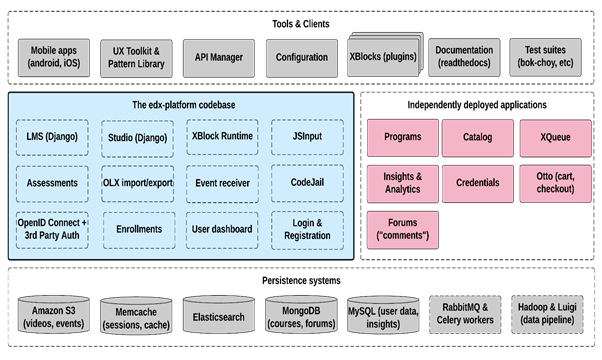
\includegraphics[width=\linewidth]{images/edx_arch_0.png}
	\caption{Open EdX Architecture}
	\label{Fig.1:Open edX Architecture}
\end{figure}

\section{Key Components}

\subsection{Learning Management System}
The Learning Management System or the LMS is the most visible part of the Open edX project.
Learners and students access their courses through the LMS and its effective functionalities makes
Open edX a efficient MOOC platform. The LMS also provides an instructor dashboard that users
who have the Admin or Staff role can access by selecting Instructor.\newline
The LMS uses a number of data stores. Courses are stored in MongoDB which is a NoSQL
Database, with videos served from YouTube or Amazon S3. Per-learner data is stored in MySQL.
As learners move through courses and interact with them, events are published to the analytics
pipeline for collection, analysis, and reporting.\newline

\subsection{Studio}
Studio is the course authoring environment. Course teams use it to create and update courses.
Studio writes its courses to the same Mongo database that the LMS uses.

\subsection{Discussions}
Course discussions are managed by an \textbf{IDA} called comments (also called forums) comments is one
of the few non-Python components, written in \textbf{Ruby} using the \textbf{Sinatra} framework. The LMS uses
an API provided by the comments service to integrate discussions into the learners’ course
experience.\newline
The comments service includes a notifier process that sends learners notifications about updates in
topics of interest.\newline

\subsection{Mobile Apps}
The Open edX project includes a mobile application, available for iOS and Android, that allows
learners to watch course videos and more. EdX is actively enhancing the mobile app.

\subsection{Analytics}
Events describing learner behavior are captured by the Open edX analytics pipeline. The events are
stored as \textbf{JSON} in S3, processed using \textbf{Hadoop}, and then digested, aggregated results are published
to \textbf{MySQL}. Results are made available via a \textbf{REST API} to Insights, an IDA that instructors and
administrators use to explore data that lets them know what their learners are doing and how their
courses are being used.

\begin{figure}
	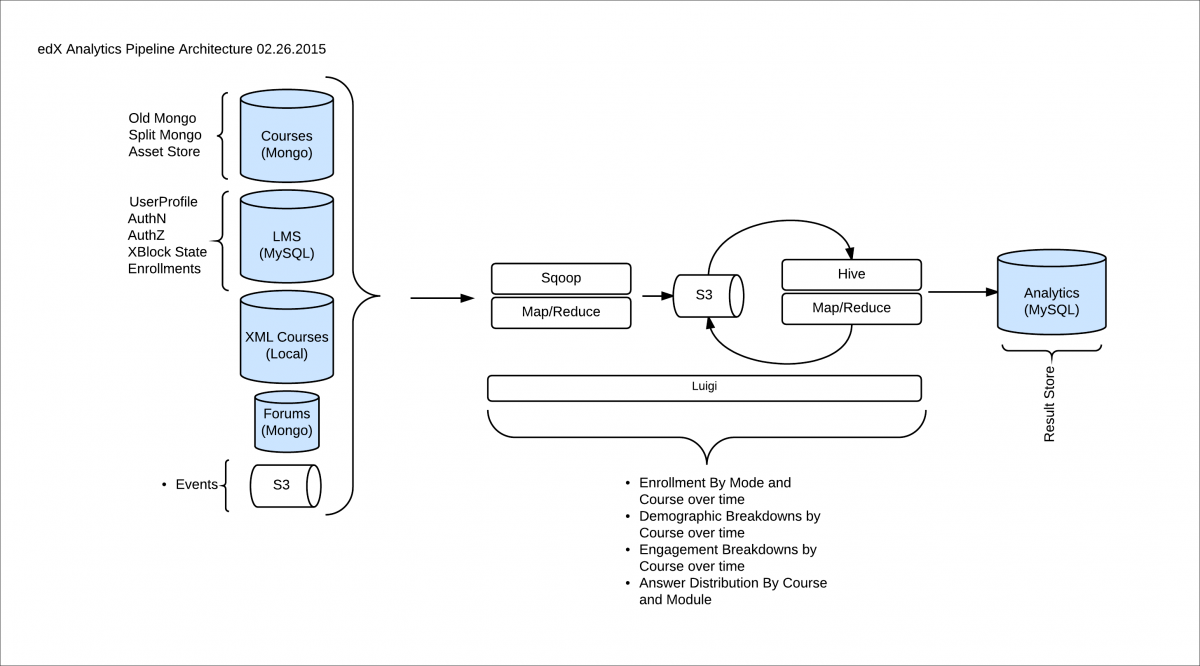
\includegraphics[width=\linewidth]{images/edx_pipeline_0.png}
	\caption{Open edX Pipeline}
	\label{Fig.2:Open edX Pipeline}
\end{figure}

\subsection{Background Work}
A number of tasks are large enough that they are performed by separate background workers, rather
than in the web applications themselves. This work is queued and distributed using \textbf{Celery} and
\textbf{RabbitMQ}. Examples of queued work include:\newline
\begin{itemize}
	\item Grading entire courses
	\item Sending bulk emails(with Amazon SES)
	\item Generating answer distribution reports
	\item Producing end-of-course certificates
\end{itemize}
The Open edX project includes an IDA called \textbf{XQueue} that can run custom graders. These are
separate processes that run compute-intensive assessments of learners’ work.

\subsection{Search}
The Open edX project uses \textbf{ElasticSearch} for searching in multiple contexts, including course
search and the comments service.

%%%%%%%%%%%%%%%%%%%%%%%%%%%%%%%%%%%%%%%%%%%%%%%

\chapter{XBlocks - The component architecture of Open edX}

\section{What is an XBlock ?}
The XBlock specification is a component architecture designed to make it easier to create new
online educational experiences. An XBlock is the basic building block of any edX course. It
controls its own data structure (\textbf{model}), its own HTML rendering (\textbf{view}), and its own business logic
(\textbf{controller}). An XBlock executes in a \textbf{runtime}, which provides common services/utilities,
user/request context, and storage. While the course structure data is primarily stored in a database
infrastucture called \textbf{modulestore}, an XBlocks \textbf{persistence} is configured on a field-by-field basis
by designating the scope or each of its \textbf{fields}. Some scopes support user-specific data, which results
in different XBlock content for different target users.\newline
An XBlock has a unique identifier known as \textbf{block-id}. Its instantiation within a context of a course
is identified by its \textbf{usage-id}. A common class of XBlocks have the same defined \textbf{type} (or \textbf{category})
that indicate its common behavior and interface. Some examples of XBlock types are:
"course\_info" (shared by Handouts and Announcements), "problem" (shared by all CAPA-based
assessments), "video", "chapter" (a.k.a Section), and "sequential" (a.k.a. Subsection).\newline
\begin{figure}
	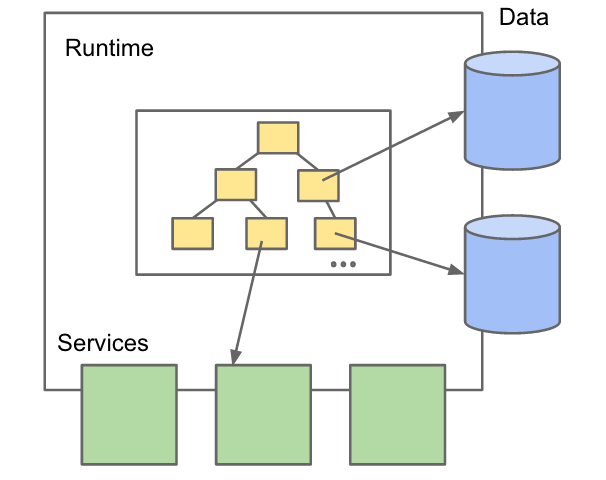
\includegraphics[width=\linewidth]{images/xblock_runtime.png}
	\caption{XBlock Runtime}
	\label{Fig.1:Xblock runtime}
\end{figure}
\section{XBlock Concepts}
XBlocks are build such that course teams use them to create independent course components that
work seamlessly with other components in an online course. These include the following\newline
\begin{itemize}
	\item \textbf{XBlock Fields : }\newline These are used to store state data for your XBlock.
	\item \textbf{XBlock Methods :}\newline These are used in the XBlock Python file to define the behavior of your XBlock.
	\item \textbf{XBlock Fragments :}\newline A fragment is a part of a web page returned by an XBlock view
method. A fragment typically contains all the resources needed to display the XBlock in a
web page, including HTML content, JavaScript, and CSS resources.
	\item \textbf{XBlock children:}\newline An XBlock can have child XBlocks.
	\item \textbf{XBlock runtime :}\newline An XBlock runtime is the application that hosts XBlock.
\end{itemize}

\section{XBlock \& edX Platform}

\subsection{EdX Studio}
EdX Studio is the application in the edX platform that instructors use to build courseware. Because
instructors use Studio to add and configure XBlocks, Studio is also an Xblock runtime application.

\subsection{EdX LMS}
The EdX Learning Management System (LMS) is the application in the edX Platform that learners
use to view and interact with courseware. Because it presents XBlocks to learners and records their
interactions, the LMS is also an Xblock runtime application.

\section{XBlock Tree Structure}
An XBlock does not refer directly to its children. Instead, the structure of a tree of XBlocks is
maintained by the runtime application, and is made available to the XBlock through a runtime
service.\newline
This allows the runtime to store, access, and modify the structure of a course without incurring the
overhead of the XBlock code itself.\newline
XBlock children are not implicitly available to their parents. The runtime provides the parent
XBlock with a list of child XBlock IDs. The child XBlock can then be loaded with the
\verb|get_child()| function. Therefore the runtime can defer loading child XBlocks until they are actually
required.

\section{Data Access \& Persistence}
\textbf{Data Access} refers to software and activities related to storing, retrieving, or acting on data housed
in a database or other repository. Two fundamental types of data access exist:
\begin{enumerate}
	\item Sequential Access
	\item Random Access
\end{enumerate}
\textbf{Persistence} refers to object and process characteristics that continue to exist even after the
process that created it ceases or the machine it is running on is powered off.

\subsection{Data Access and Persistence in edX platform}
This part describes how the edx-platform does CRUD (Create, Read, Update, Delete) operations on
xblocks and other models and backs those operations with persistence. Currently Open edX uses
Django's ORM backed by a SQL DB as the persistence layer for user-relative data. The user history
data is moved to a non-SQL db(Mongo db).

\subsection{XMLModuleStore}
\begin{itemize}
	\item The original course data is in xml which is stored on a file system
	\item When the server launches, it scans the file systen and loads every such course into memory
	\item It then serves the courseware from memory
	\item The \textbf{XMLModuleStore} is the data access layer which finds, loads and serves up the course data to the application. It has only read access. NO create, update NOR delete.
\end{itemize}

\subsection{MongoModuleStore}
\begin{itemize}
	\item When Studio is launched, a read-write storage mechanism and data access layer is needed
so, \textbf{MongoModuleStore} with CRUD methods is added.
	\item Here the persistence technology (Mongo) with the DAO CRUD functionality has been
convoluted
	\item \textbf{MongoModuleStore} stores each Xmodule as a separate document in a non-SQL (Mongo)
database.
	\item The db connection and pymongo usages are needed to be abstracted out. Hence it uses the
xblock's old style location (tag, org, courseid, type, blockid, draft or None) as the key.
	\item All changes (add, remove, move child) immediately impact the published course.
	\item \textbf{MongoModuleStore} handles inheritance by loading the whole course on each access.
\end{itemize}

\subsection{SplitMongoModuleStore}
\begin{itemize}
	\item It is created to fix the expense and fragility of inheritance.
	\item It offers full versioning of all edits, the ability to share the same content and settings between
courses, as many named branches of a course or named-subcourse structure as one needs.
	\item Once again the persistence technology (Mongo) with the DAO functionality (CRUD operations
on xblocks) is being convoluted.
\end{itemize}


%%%%%%%%%%%%%%%%%%%%%%%%%%%%%%%%%%%%%%%%%%%%%%%

\chapter{HTML Component in Open edX}

\section{What is an HTML editor}

An \textbf{HTML editor} is a program for editing HTML, the markup of a webpage. HTML can be written
with any text editor but specialized HTML editors can offer convenience and added functionality.
For example, many HTML editors handle not only HTML, but also related technologies such
as CSS , XML and JavaScript. In some cases they also manage communication with remote web
servers via FTP and WebDAV, and version control system such as Subversion or Git.

\section{HTML component in Open edX}
\begin{itemize}
	\item HTML components are the basic building blocks of the course content.
	\item These are used for adding and formatting text, links, images and much more.
	\item One can work with the HTML components in a “visual ” or WYSIWYG editor that hides the
HTML code details, or in a “raw” editor that is required to mark up the content.
\end{itemize}
The Open edX platform uses the following three JavaScript editors presently :-
\begin{enumerate}
	\item TinyMCE
	\item CodeMirror
	\item WMD
\end{enumerate}

\section{Options for editing HTML components}
To work with HTML component, two different editing interfaces can be used.
\begin{itemize}
	\item \textbf{Visual Editor (TinyMCE) }
		\begin{enumerate}
			\item This interface is almost similar to the interface of “MS Word”.
			\item Using the visual editor one can create, edit, add links \& images and format content
without using HTML markup directly.
			\item The visual editor includes an HTML option for reviewing the HTML markup and can
make any changes to the content if we want
		\end{enumerate}
	\item \textbf{Raw HTML Editor (CodeMirror) }
		\begin{enumerate}
			\item It is a text editor and it does not offer a toolbar with formatting options.
			\item This is used to markup content directly with HTML markup.
			\item To include custom formatting or scripts in the course content, a raw HTML editor
is needed.
		\end{enumerate}
\end{itemize}

\section{Current scenario of Open edX HTML Editors}

\subsection{TinyMCE}
\begin{itemize}
	\item Version 4.0.20(from March 2013). Version 4.7.13 is available as of May 2018
	\item Where is it used :
		\begin{enumerate}
			\item WYSIWYG editing of HTML course content in studio
			\item Bulk email in the instructor dashboard
		\end{enumerate}
	\item Plugins used :
		\begin{enumerate}
			\item "CodeMirror-For-TinyMCE" which allows TinyMCE to interoperate with CodeMirror
			\item "Spell checker"
			\item A studio skin for TinyMCE has also been written.
		\end{enumerate}
	\item Challenges involved in updating :
		\begin{enumerate}
			\item The installed version of TinyMCE is very old
			\item It is not accessible (Accessible here means accessibility to browser screen readers.)
			\item There are large number of edX specific modifications that will be harder to migrate
		\end{enumerate}
\end{itemize}

\subsection{CodeMirror}
\begin{itemize}
	\item Version 3.15(from February 2014). Version 5.38.0 is available as of May 2018
	\item Where is it used :
		\begin{enumerate}
			\item Code editing
			\item Raw HTML editor in studio
			\item XML code for authoring studio's advanced editor for problems
			\item JSON in studio's advanced settings
			\item Python (and other languages) code for externally graded assessments in the LMS
		\end{enumerate}
	\item Challenges involved in updating :
		\begin{enumerate}
			\item The installed version of CodeMirror is very old
			\item It may not be accessible
			\item CodeMirror has issues with right-to-left layouts, and even the most recent version doesn't seem to address it.
		\end{enumerate}
\end{itemize}

\subsection{WMD}
\begin{itemize}
	\item Version unknown(edX forked the code in 2012)
	\item Where is it used ? It is used as markdown editor for discussion posts
	\item Challenges involed in updating :
		\begin{enumerate}
			\item WMD/PageDown is a dead project
			\item WMD is not fully accessible
			\item There are a lot of custom edX modifications that will be hard to support going forward
		\end{enumerate}
\end{itemize}

%%%%%%%%%%%%%%%%%%%%%%%%%%%%%%%%%%%%%%%%%%%%%%%
